\documentclass[11pt]{article}
\usepackage[a4paper,margin=2.1cm]{geometry}
\usepackage{amsmath,amssymb,booktabs,array,longtable,microtype,xcolor,hyperref,tikz}
\usetikzlibrary{arrows.meta,positioning,calc,shapes.geometric}
\hypersetup{colorlinks=true,linkcolor=blue!50!black,urlcolor=blue!50!black,citecolor=blue!50!black}
\definecolor{mmalsblue}{RGB}{32,86,140}
\definecolor{mmalsgreen}{RGB}{46,125,92}
\definecolor{mmalsorange}{RGB}{190,110,20}
\newcommand{\OT}{\operatorname{OT}}
\title{\textbf{Geometry-MMALS G1 v1.1.3}\\Functional Memory Transport, Route-Path Diagnostics, and Limited-Replay Retention}
\author{MMALS Research Program\\Guillaume Harbonnier}
\date{June 2026\\C0 specification -- empirical pilot pending}
\begin{document}
\maketitle
\begin{abstract}
Geometry-MMALS G1 v1.1.1 isolated the context-to-route bridge under one frozen host ecosystem. Version 1.1.2 repaired the sharp local tails of prototype routing but did not outperform the low-capacity linear router on held-out functional order or stress. Covariance-aware context geometry nevertheless added stable information beyond centroid-only geometry. Version 1.1.3 therefore fixes one linear router architecture and tests a different hypothesis: which memory object should constrain the route as learning proceeds? The protocol compares current-only learning, limited replay, nominal route anchoring, functional transport anchoring under a frozen host-cost matrix, and a joint functional-memory objective. It measures paired and distributional transport, latent and output drift, identity preservation, route-path length, endpoint drift, path excess, and a diagnostic compressed memory in root-simplex coordinates. The claim is intentionally narrow: v1.1.3 can test whether functional transport preserves old behavior more efficiently than nominal route anchoring under a fixed ecosystem and fixed memory budget.
\end{abstract}
\tableofcontents
\section{Motivation from v1.1.2}
The v1.1.2 pilot showed that R5 improved held-out functional geometry over the MLP baseline but not robustly over the linear router. Its continuity repair worked mechanically, while the covariance-aware context diagnostic improved stress over centroid-only geometry by $-0.0442$ with a five-seed confidence interval entirely below zero. The next experiment therefore stops adding router capacity and asks whether the correct route-function memory object is being preserved.

\section{Frozen experimental ecosystem}
For every seed, all treatments share and freeze
\[
z_0=P(x),\qquad c=C_\phi(z_0),\qquad u_h=g_h(z_0),
\]
\[
z_M(r)=\sum_{h=1}^{H}r_hu_h,\qquad \hat y=Q(z_M),
\]
including the sensory encoder, context encoder, host bank, synthesis normalization, classifier, and common host-cost matrix $C^\star$. Only a linear router is trainable:
\[
r_\theta(c)=\operatorname{softmax}(Wc+b).
\]

\begin{figure}[h]
\centering
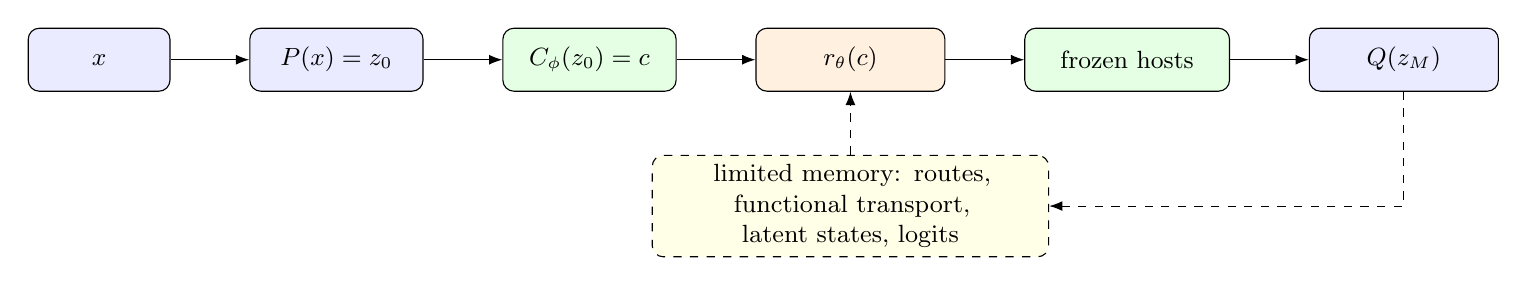
\begin{tikzpicture}[node distance=7mm and 10mm,>=Latex, every node/.style={font=\small}]
\node[draw,rounded corners,fill=blue!8,minimum width=18mm,minimum height=8mm] (x) {$x$};
\node[draw,rounded corners,fill=blue!8,right=of x,minimum width=22mm,minimum height=8mm] (p) {$P(x)=z_0$};
\node[draw,rounded corners,fill=green!10,right=of p,minimum width=22mm,minimum height=8mm] (c) {$C_\phi(z_0)=c$};
\node[draw,rounded corners,fill=orange!12,right=of c,minimum width=24mm,minimum height=8mm] (r) {$r_\theta(c)$};
\node[draw,rounded corners,fill=green!10,right=of r,minimum width=26mm,minimum height=8mm] (h) {frozen hosts};
\node[draw,rounded corners,fill=blue!8,right=of h,minimum width=24mm,minimum height=8mm] (q) {$Q(z_M)$};
\draw[->] (x)--(p);\draw[->] (p)--(c);\draw[->] (c)--(r);\draw[->] (r)--(h);\draw[->] (h)--(q);
\node[below=8mm of r,draw,dashed,rounded corners,fill=yellow!10,text width=48mm,align=center] (mem) {limited memory: routes, functional transport, latent states, logits};
\draw[->,dashed] (q.south) |- (mem.east);
\draw[->,dashed] (mem.north) -- (r.south);
\end{tikzpicture}
\caption{The v1.1.3 experiment changes the memory objective while keeping the entire functional ecosystem and router architecture fixed.}
\end{figure}

\section{Route-function memory object}
For source $x$, regime $u$, and stage $t$,
\[
\Phi_t(x,u)=\bigl(r_t,z_{M,t},p_t\bigr),
\]
where $r_t$ is the route, $z_{M,t}$ is the mediated latent state, and $p_t$ is the output distribution. The original stage snapshot is frozen when a regime is first learned; later stages cannot redefine the teacher.

\section{Limited replay protocol}
Each stage receives the current-angle training subset and exactly 64 remembered source identities per previous angle. No other historical training examples are available. Memory identities, batch schedules, optimizer steps, and forward counts are identical across treatments. Final drift is evaluated on source-disjoint test identities by comparing the final model to the original stage snapshot.

\section{Treatments}
\begin{center}
\begin{tabular}{lcccccc}
\toprule
Treatment & Current CE & Replay CE & Route & Functional OT & Latent & Output KL\\
\midrule
M0 current only & yes & no & no & no & no & no\\
M1 replay CE & yes & yes & no & no & no & no\\
M2 route anchor & yes & yes & yes & no & no & no\\
M3 functional transport & yes & yes & no & yes & no & no\\
M4 joint functional memory & yes & yes & no & yes & yes & yes\\
\bottomrule
\end{tabular}
\end{center}

\section{Memory losses}
Nominal route anchoring uses square-root simplex coordinates:
\[
\mathcal L_R=\frac{1}{2B}\sum_n\left\|\sqrt{r_t^{(n)}}-\sqrt{r_{\rm ref}^{(n)}}\right\|_2^2.
\]
The common host cost is
\[
C^\star_{hk}=\mathbb E_x\frac{\|g_h(P(x))-g_k(P(x))\|_2^2}{d_M}.
\]
Functional route transport is
\[
\mathcal L_F=\frac{1}{B}\sum_n\OT_{C^\star}\left(r_t^{(n)},r_{\rm ref}^{(n)}\right).
\]
Latent and output preservation are
\[
\mathcal L_Z=\frac1B\sum_n\|z_{M,t}^{(n)}-z_{M,\rm ref}^{(n)}\|_2^2,
\]
\[
\mathcal L_Y=T^2\operatorname{KL}\!\left(\operatorname{softmax}(\ell_{\rm ref}/T)\,\|\,\operatorname{softmax}(\ell_t/T)\right).
\]

\section{Distributional transport}
For an old angle $u$,
\[
\mu_{u,t}=\frac1N\sum_n\delta_{r_t(x_n,u)}.
\]
The whole-memory movement is
\[
\mathcal T_u^{t-1\rightarrow t}=\inf_{\gamma\in\Pi(\mu_{u,t-1},\mu_{u,t})}\sum_{ij}\gamma_{ij}\,d_{C^\star}(r_i,r_j).
\]
This complements source-matched drift by asking whether the entire route distribution moved.

\section{Path diagnostics}
For an old regime $u$,
\[
L_u=\sum_{s=u+1}^{T}d_F(\mu_{u,s-1},\mu_{u,s}),\qquad D_u=d_F(\mu_{u,u},\mu_{u,T}),
\]
\[
E_u=\frac{L_u}{D_u+\varepsilon}.
\]
$E_u$ detects oscillatory or wasteful movement even when the final endpoint returns near the original memory.

\begin{figure}[h]
\centering
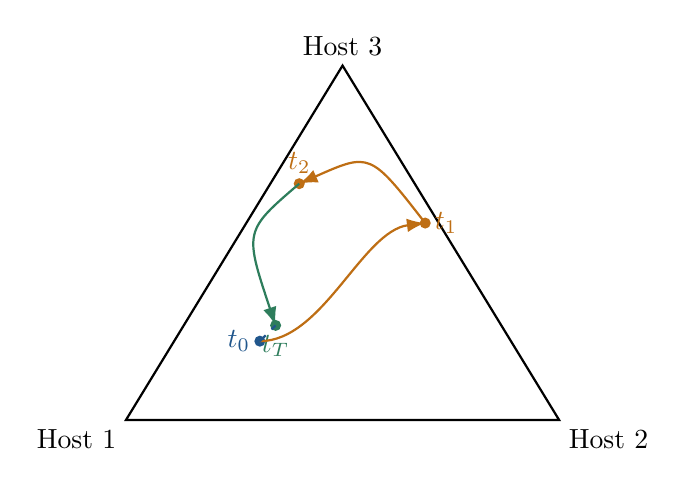
\begin{tikzpicture}[scale=1.0,>=Latex]
\draw[thick] (0,0)--(5.5,0)--(2.75,4.5)--cycle;
\node[below left] at (0,0) {Host 1};\node[below right] at (5.5,0) {Host 2};\node[above] at (2.75,4.5) {Host 3};
\coordinate (a) at (1.7,1.0);\coordinate (b) at (3.8,2.5);\coordinate (c) at (2.2,3.0);\coordinate (d) at (1.9,1.2);
\fill[mmalsblue] (a) circle (2pt) node[left] {$t_0$};
\fill[mmalsorange] (b) circle (2pt) node[right] {$t_1$};
\fill[mmalsorange] (c) circle (2pt) node[above] {$t_2$};
\fill[mmalsgreen] (d) circle (2pt) node[below] {$t_T$};
\draw[->,thick,mmalsorange] (a).. controls (2.5,1.0) and (3.0,2.4)..(b);
\draw[->,thick,mmalsorange] (b).. controls (3.1,3.4) ..(c);
\draw[->,thick,mmalsgreen] (c).. controls (1.5,2.4) ..(d);
\draw[dashed,thick,mmalsblue] (a)--(d);
\end{tikzpicture}
\caption{Endpoint drift can be small while cumulative path length is large. Path excess exposes such hidden memory motion.}
\end{figure}

\section{Compiled memory diagnostic}
A compressed memory stores a Gaussian summary of root routes,
\[
q_u=\mathcal N(m_u,\Sigma_u),\qquad m_u=\mathbb E[\sqrt r],\qquad \Sigma_u=\operatorname{Cov}(\sqrt r)+\epsilon I.
\]
Held-out negative log-likelihood under the covariance-aware summary is compared with an isotropic or barycenter-only summary. This is a diagnostic and does not replace replay in the primary experiment.

\section{Primary gates}
\subsection*{A. Functional transport versus route anchoring}
M3 qualifies over M2 only if the five-seed confidence interval for endpoint functional drift is entirely favorable and at least four of five seeds improve.
\subsection*{B. Joint functional memory versus replay}
M4 qualifies over M1 only if old-angle forgetting is lower with an entirely favorable seed confidence interval and at least four of five favorable seeds.
\subsection*{Safety}
The frozen ecosystem, matched compute, exact memory budget, source-disjoint evaluation, prediction identity, and new-angle accuracy margin are mandatory. Failure of a protocol-integrity gate blocks the corresponding scientific claim.

\section{Required evidence}
The notebook exports split and memory manifests, hashes, memory budgets, staged accuracy, paired and distributional transport, latent drift, output KL, identity, path statistics, compiled-memory diagnostics, aggregate seed effects, gates, run and claim manifests, and environment capture.

\section{Interpretation discipline and roadmap}
A positive pilot would support only the claim that functional transport preserves old route-function behavior better than nominal route anchoring or replay under a fixed ecosystem and fixed memory budget. It would not establish mature host specialization, positive backward transfer, operational superiority, optimality of the transport, a learned Riemannian manifold, reinforcement-learning control, or quantum advantage. The next branch is v1.1.4 selective causal host adaptation and recovery, followed by explicit bottom-up host feedback and TPUT goal-conditioned control.
\end{document}
